%Type of Document
\documentclass[a4paper, 12pt]{report}

%Load Pre-ambles
\usepackage{../../Environment/Packages}
\usepackage{../../Environment/Conventions}
\usepackage{../../Environment/Hyahoos}
\def\sized{0.14}

\begin{document}

\begin{center}
%Seperator
%Seperator
%Seperator
%Seperator
%Seperator
\section{Fourier Stability Analysis}
\begin{comment}
\end{comment}
%Seperator
%Seperator
%Seperator
\subsection{Discretization of Wave Equation}
\begin{comment}
\end{comment}
The one-dimensional wave equation is shown below,
$$0 = \f{\p\phi}{\p t} + u\f{\p\phi}{\p x}$$
Integrating with time and space,
$$0 = \int^{t+\Delta t}_{t}\int_{CV} \f{\p\phi}{\p t} \,dVdt + u\int^{t+\Delta t}_{t}\int_{CV}\f{\p\phi}{\p x}\,dVdt$$
Switching the order of integration in order to form exact differentials,
$$0 = \int_{CV}\int^{t+\Delta t}_{t} \f{\p\phi}{\p t} \,dt\,dV + u\int^{t+\Delta t}_{t}\int_{CV}\f{\p\phi}{\p x}\,dVdt$$
$$0 = \int_{CV}\l[\phi\r]^{t+\Delta t}_{t} \,dV + u\int^{t+\Delta t}_{t}A\l[\phi\r]_{CV}\,dt$$
$$0 = \l[\phi\r]^{t+\Delta t}_{t}\Delta V  + u\int^{t+\Delta t}_{t}A\phi_{e} - A\phi_{w}\,dt$$
Substituting for the infinitesmially small volume $\Delta V = A dx$,
$$0 = \l[\phi\r]^{t+\Delta t}_{t}A dx  + u\int^{t+\Delta t}_{t}A\phi_{e} - A\phi_{w}\,dt$$
Assuming uniform area throughout the grids,
$$0 = \l[\phi\r]^{t+\Delta t}_{t} dx  + u\int^{t+\Delta t}_{t}\phi_{e} - \phi_{w}\,dt$$
Assuming that the value of $\phi$ is constant within a single cell,
$$0 = \l[\phi_{P} - \phi_{P,o}\r] dx  + u\int^{t+\Delta t}_{t}\phi_{e} - \phi_{w}\,dt$$
Using the generalized time integration scheme,
$$\int^{t+\Delta t}_{t} \phi\,dt = [\t\phi_{t+\Delta t} + (1-\t)\phi_{t}]\Delta t$$
Substituting the time integration scheme,
$$0 = \l[\phi_{P} - \phi_{P,o}\r] dx  + u\l\{\t\phi_{e} + (1-\t)\phi_{e,o} - \t\phi_{w} - (1-\t)\phi_{w,o}\r\}dt$$
Factoring for the CFL number,
$$0 = \l[\phi_{P} - \phi_{P,o}\r] \f{dx}{u\,dt}  + \l\{\t\phi_{e} + (1-\t)\phi_{e,o} - \t\phi_{w} - (1-\t)\phi_{w,o}\r\}$$
$$0 = \l[\phi_{P} - \phi_{P,o}\r] \f{\Delta x}{u\,\Delta t}  + \t\phi_{e} + (1-\t)\phi_{e,o} - \t\phi_{w} - (1-\t)\phi_{w,o}$$
Let 
$$\g = \f{1}{CFL} = \f{\Delta x}{u\,\Delta t}$$
$$0 = \g\phi_{P} - \g\phi_{P,o}   + \t\phi_{e} + (1-\t)\phi_{e,o} - \t\phi_{w} - (1-\t)\phi_{w,o}$$
Placing the new time step quantities on $LHS$ and the old time step quantities on $RHS$,
$$-\g\phi_{P} + \t\phi_{w} - \t\phi_{e} = - \g\phi_{P,o} + (1-\t)\phi_{e,o} - (1-\t)\phi_{w,o}$$
%Seperator
%Seperator
\subsection{Cubic Polynomial Spatial Scheme}
\begin{comment}
\end{comment}

The discretization of the pure convection problem with a generalized time advancement scheme and a cubic polynomial spatial advancement scheme is shown below,
\begin{equation*}
\begin{split}
%Seperator
0 =\,\, &\f{\phi_{P} - \phi_{P,o}}{\Delta t} + \f{u}{\Delta x}\l[ \t\l(\f{1}{16}\phi_{WW} - \f{5}{16}\phi_{W} + \f{15}{16}\phi_{P} + \f{5}{16}\phi_{E}\r) \right.
%Seperator
\\ & + (1-\t)\l( \f{1}{16}\phi_{WW,o} - \f{5}{16}\phi_{W,o} + \f{15}{16}\phi_{P,o} + \f{5}{16}\phi_{E,o}\r)
%Seperator
\\ & -\t \l( \f{1}{16}\phi_{WWW} - \f{5}{16}\phi_{WW} + \f{15}{16}\phi_{W} + \f{5}{16}\phi_{P}\r)
%Seperator
\\ & \left. - (1-\t)\l( \f{1}{16}\phi_{WWW,o} - \f{5}{16}\phi_{WW,o} + \f{15}{16}\phi_{W,o} + \f{5}{16}\phi_{P,o}\r)\r]
%Seperator
\end{split}
\end{equation*}


Assuming that the solution $\phi(x,t)$ is a product of a time component $\h{\phi}(t)$ and a spatial component $e^{ikx}$, the solution $\phi(x,t)$ could be rewritten as,
$$\phi(x,t) = \h{\phi}(t)e^{ikx}$$


Points at the future time step would be given the time component shown below,
$$\h{\phi}(t+\Delta t) = \h{\phi}$$
Points at the old time step would be given the time component shown below,
$$\h{\phi}(t) = \h{\phi}_o$$

Following convention, the coordinate system considers eastern direction of the grid points to be positive $x$ and western direction of the grid points to be negative $x$. The point of interest $P$ would be given a spatial component $e^{ikx}$. Following the coordinate system definition, the west point would be given spatial component $e^{ik(x-\Delta x)}$. The east point would be given spatial component $e^{ik(x+\Delta x)}$. The diagram below summarizes the coordinate system used in this derivation,
%\\~\\~\\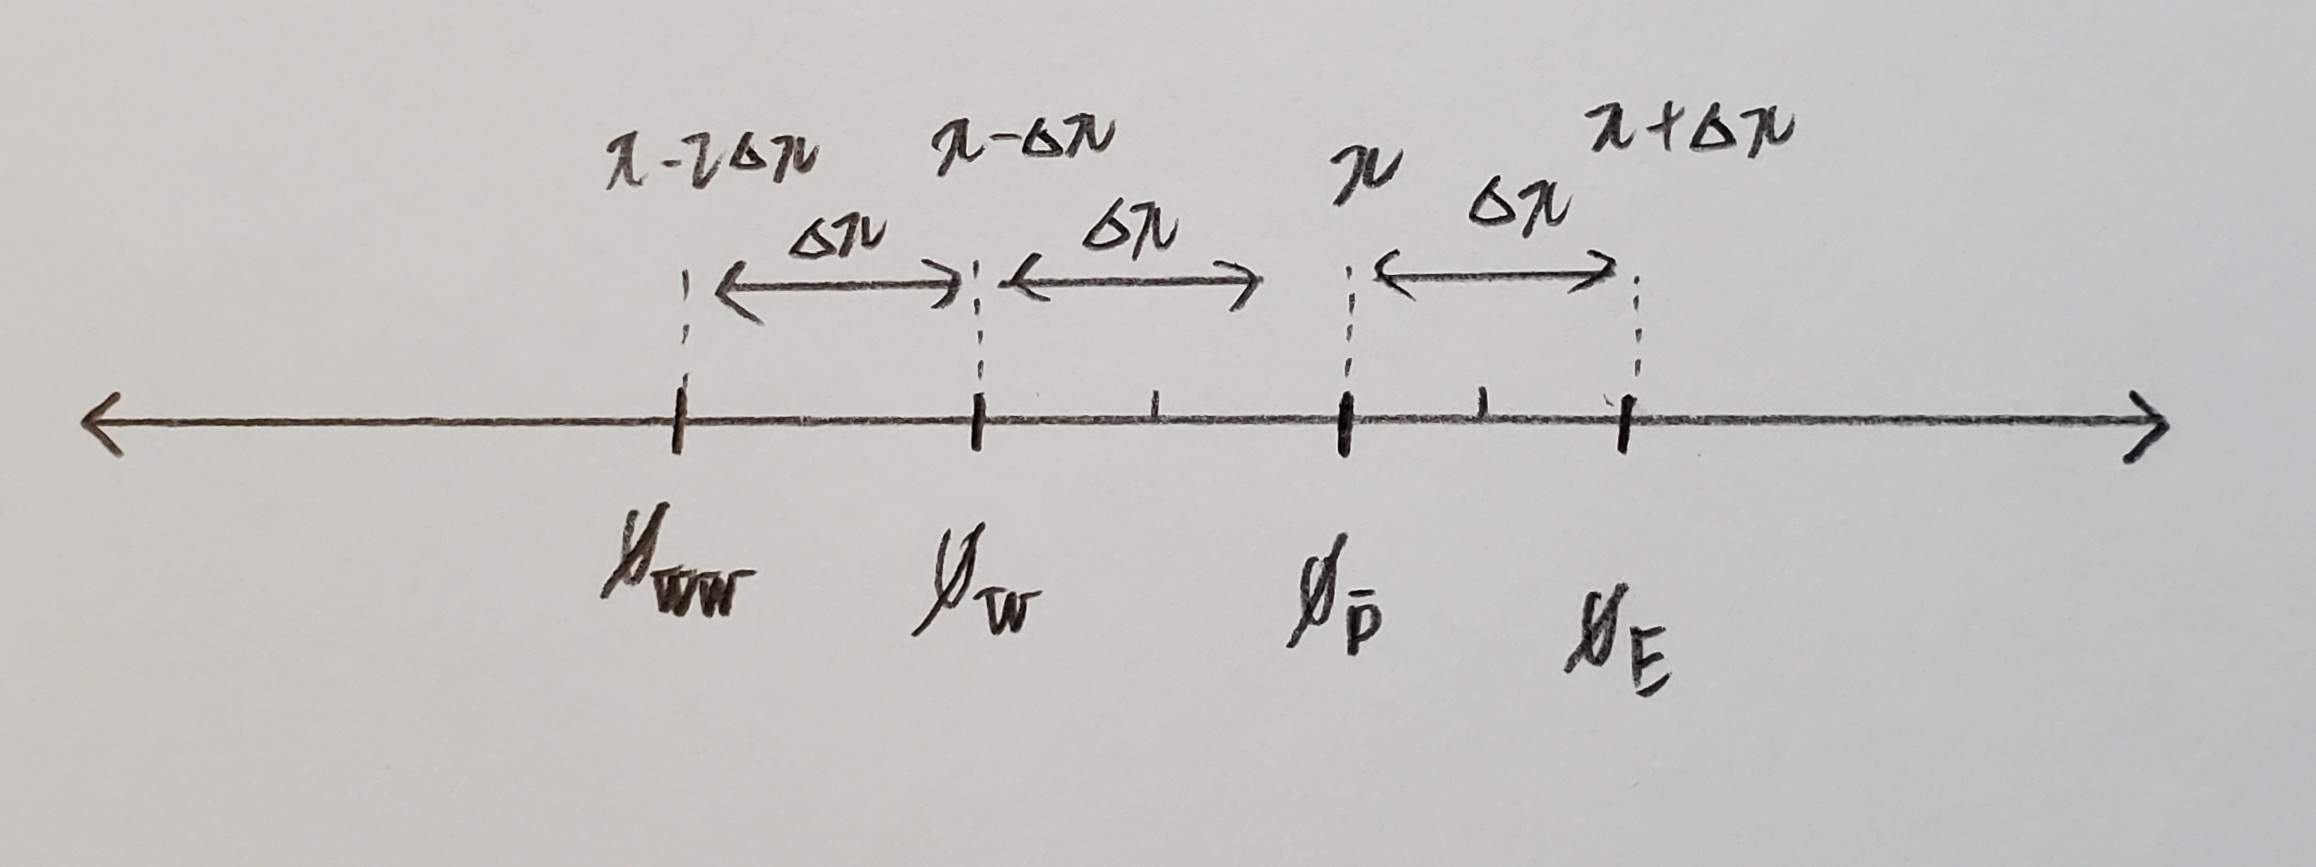
\includegraphics[scale=\sized]{Mambah.jpg}
\\~\\~\\Uniform grid spacing is assumed in the following derivation. Parsing the original expression into several parts. 
For the discrete derivative of $\phi$ with respect to time,
$$\f{\phi_{P} - \phi_{P,o}}{\Delta t} = \f{1}{\Delta t}\l[\phi_{P} - \phi_{P,o}\r] = \f{1}{\Delta t}\l[\h{\phi}e^{ikx} - \h{\phi}_oe^{ikx}\r] = \f{e^{ikx}}{\Delta t}\l[\h{\phi} - \h{\phi}_o\r]$$

For the first part of $RHS$,
\begin{equation*}
\begin{split}
%Seperator
\f{1}{16}\phi_{WW} - \f{5}{16}\phi_{W} + \f{15}{16}\phi_{P} + \f{5}{16}\phi_{E} = & \f{1}{16}\h{\phi}e^{ik(x - 2\Delta x)} - \f{5}{16}\h{\phi}e^{ik(x - \Delta x)}       
%Seperator
\\ &+ \f{15}{16}\h{\phi}e^{ikx} + \f{5}{16}\h{\phi}e^{ik(x + \Delta x)}
%Seperator
\end{split}
\end{equation*}
\begin{equation*}
\begin{split}
%Seperator
\f{1}{16}\phi_{WW} - \f{5}{16}\phi_{W} + \f{15}{16}\phi_{P} + \f{5}{16}\phi_{E} = & \f{1}{16}\h{\phi}e^{ikx - 2ik\Delta x} - \f{5}{16}\h{\phi}e^{ikx - ik\Delta x}       
%Seperator
\\ &+ \f{15}{16}\h{\phi}e^{ikx} + \f{5}{16}\h{\phi}e^{ikx + ik\Delta x}
%Seperator
\end{split}
\end{equation*}
\begin{equation*}
\begin{split}
%Seperator
\f{1}{16}\phi_{WW} - \f{5}{16}\phi_{W} + \f{15}{16}\phi_{P} + \f{5}{16}\phi_{E} = & \f{1}{16}\h{\phi}e^{ikx}e^{-2ik\Delta x} - \f{5}{16}\h{\phi}e^{ikx}e^{-ik\Delta x}       
%Seperator
\\ &+ \f{15}{16}\h{\phi}e^{ikx} + \f{5}{16}\h{\phi}e^{ikx}e^{ik\Delta x}         
%Seperator
\end{split}
\end{equation*}
$$\f{1}{16}\phi_{WW} - \f{5}{16}\phi_{W} + \f{15}{16}\phi_{P} + \f{5}{16}\phi_{E} = \h{\phi}e^{ikx}\l[\f{1}{16}e^{-2ik\Delta x} - \f{5}{16}e^{-ik\Delta x} + \f{15}{16} + \f{5}{16}e^{ik\Delta x}\r]$$ 

Performing similar opeartions for the second part of $RHS$,
$$\f{1}{16}\phi_{WW,o} - \f{5}{16}\phi_{W,o} + \f{15}{16}\phi_{P,o} + \f{5}{16}\phi_{E,o} = \h{\phi}_oe^{ikx}\l[\f{1}{16}e^{-2ik\Delta x} - \f{5}{16}e^{-ik\Delta x} + \f{15}{16} + \f{5}{16}e^{ik\Delta x}\r]$$

Performing similar opeartions for the third part of $RHS$,
$$\f{1}{16}\phi_{WWW} - \f{5}{16}\phi_{WW} + \f{15}{16}\phi_{W} + \f{5}{16}\phi_{P} = \h{\phi}e^{ikx}\l[\f{1}{16}e^{-3ik\Delta x} - \f{5}{16}e^{-2ik\Delta x} + \f{15}{16}e^{-ik\Delta x} + \f{5}{16}\r]$$

Performing similar opeartions for the fourth part of $RHS$,$$\f{1}{16}\phi_{WWW,o} - \f{5}{16}\phi_{WW,o} + \f{15}{16}\phi_{W,o} + \f{5}{16}\phi_{P,o} = \h{\phi}_oe^{ikx}\l[\f{1}{16}e^{-3ik\Delta x} - \f{5}{16}e^{-2ik\Delta x} + \f{15}{16}e^{-ik\Delta x} + \f{5}{16}\r]$$
   
Let$$A = \f{1}{16}e^{-2ik\Delta x} - \f{5}{16}e^{-ik\Delta x} + \f{15}{16} + \f{5}{16}e^{ik\Delta x} \quad,\quad B = \f{1}{16}e^{-3ik\Delta x} - \f{5}{16}e^{-2ik\Delta x} + \f{15}{16}e^{-ik\Delta x} + \f{5}{16}$$

Substituting for $A$ and $B$ shortens the expressions,
$$\f{1}{16}\phi_{WW} - \f{5}{16}\phi_{W} + \f{15}{16}\phi_{P} + \f{5}{16}\phi_{E} = \h{\phi}e^{ikx}A$$
$$\f{1}{16}\phi_{WW,o} - \f{5}{16}\phi_{W,o} + \f{15}{16}\phi_{P,o} + \f{5}{16}\phi_{E,o} = \h{\phi}_oe^{ikx}A$$
$$\f{1}{16}\phi_{WWW} - \f{5}{16}\phi_{WW} + \f{15}{16}\phi_{W} + \f{5}{16}\phi_{P} = \h{\phi}e^{ikx}B$$
$$\f{1}{16}\phi_{WWW,o} - \f{5}{16}\phi_{WW,o} + \f{15}{16}\phi_{W,o} + \f{5}{16}\phi_{P,o} = \h{\phi}_oe^{ikx}B$$

Susbtituting the simplified parts into the original expression,
$$0 = \f{e^{ikx}}{\Delta t}\l[\h{\phi} - \h{\phi}_o\r] + \f{u}{\Delta x}\l[\t\l(\h{\phi}e^{ikx}A\r) + (1-\t)\l(\h{\phi}_oe^{ikx}A\r) - \t\l(\h{\phi}e^{ikx}B\r) - (1-\t)\l(\h{\phi}_oe^{ikx}B\r)\r]$$
$$0 = \f{e^{ikx}}{\Delta t}\l[\h{\phi} - \h{\phi}_o\r] + \f{u}{\Delta x}\l[\t\h{\phi}e^{ikx}A + (1-\t)\h{\phi}_oe^{ikx}A - \t\h{\phi}e^{ikx}B - (1-\t)\h{\phi}_oe^{ikx}B\r]$$
Since $e^{ikx}\neq 0$,
$$0 = \f{1}{\Delta t}\l[\h{\phi} - \h{\phi}_o\r] + \f{u}{\Delta x}\l[\t\h{\phi}A + (1-\t)\h{\phi}_oA - \t\h{\phi}B - (1-\t)\h{\phi}_oB\r]$$
$$0 = \f{\Delta x}{u\,\Delta t}\l[\h{\phi} - \h{\phi}_o\r] + \t\h{\phi}A + (1-\t)\h{\phi}_oA - \t\h{\phi}B - (1-\t)\h{\phi}_oB$$
Let 
$$\g = \f{1}{CFL} = \f{\Delta x}{u\,\Delta t}$$
Substituting for the parameter $\g$,
$$0 = \g\h{\phi} - \g\h{\phi}_o + \t\h{\phi}A + (1-\t)\h{\phi}_oA - \t\h{\phi}B - (1-\t)\h{\phi}_oB$$
$$\g\h{\phi}_o - (1-\t)\h{\phi}_oA + (1-\t)\h{\phi}_oB = \g\h{\phi} + \t\h{\phi}A - \t\h{\phi}B$$
$$\h{\phi}\l[\g + \t A - \t B\r] = \h{\phi}_o\l[\g - (1-\t)A + (1-\t)B\r]$$
$$\f{\h{\phi}}{\h{\phi}_o} = \f{\l[\g - (1-\t)A + (1-\t)B\r]}{\l[\g + \t A - \t B\r]} = \f{\g + (\t-1)A + (1-\t)B}{\g + \t A - \t B} = \f{\g + \t A - A + B-\t B}{\g + \t A - \t B}$$
$$\f{\h{\phi}}{\h{\phi}_o} = \f{\g - A + B + \t A - \t B}{\g + \t A - \t B} = \f{\g - (A - B) + \t(A - B)}{\g + \t(A - B)}$$

Let $\a = A-B$. Simplifying,
$$\a = \f{1}{16}e^{-2ik\Delta x} - \f{5}{16}e^{-ik\Delta x} + \f{15}{16} + \f{5}{16}e^{ik\Delta x} - \l(\f{1}{16}e^{-3ik\Delta x} - \f{5}{16}e^{-2ik\Delta x} + \f{15}{16}e^{-ik\Delta x} + \f{5}{16}\r)$$
$$\a = \f{1}{16}e^{-2ik\Delta x} - \f{5}{16}e^{-ik\Delta x} + \f{15}{16} + \f{5}{16}e^{ik\Delta x} - \f{1}{16}e^{-3ik\Delta x} + \f{5}{16}e^{-2ik\Delta x} - \f{15}{16}e^{-ik\Delta x} - \f{5}{16}$$
$$\a = - \f{1}{16}e^{-3ik\Delta x} + \f{1}{16}e^{-2ik\Delta x} + \f{5}{16}e^{-2ik\Delta x} - \f{5}{16}e^{-ik\Delta x} - \f{15}{16}e^{-ik\Delta x} - \f{5}{16} + \f{15}{16} + \f{5}{16}e^{ik\Delta x}$$
$$\a = - \f{1}{16}e^{-3ik\Delta x} + \l[\f{1}{16} + \f{5}{16}\r]e^{-2ik\Delta x} - \l[\f{5}{16} + \f{15}{16}\r]e^{-ik\Delta x}  - \f{5}{16} + \f{15}{16} + \f{5}{16}e^{ik\Delta x}$$
$$\a = - \f{1}{16}e^{-3ik\Delta x} + \l[\f{6}{16}\r]e^{-2ik\Delta x} - \l[\f{20}{16}\r]e^{-ik\Delta x} + \f{10}{16} + \f{5}{16}e^{ik\Delta x}$$
$$\a = - \f{1}{16}e^{-3ik\Delta x} + \f{6}{16}e^{-2ik\Delta x} - \f{20}{16}e^{-ik\Delta x} + \f{10}{16} + \f{5}{16}e^{ik\Delta x}$$

Substituting for $\a$,
$$\f{\h{\phi}}{\h{\phi}_o} = \f{\g - \a + \t\a}{\g + \t\a}$$


%Seperator
%Seperator
\subsection{Upwind Differencing Scheme}
The theoretical section shows that discretizing the $1$-dimensional wave equation yields the following expression,
$$-\g\phi_{P} + \t\phi_{w} - \t\phi_{e} = - \g\phi_{P,o} + (1-\t)\phi_{e,o} - (1-\t)\phi_{w,o}$$
Assuming upwing differencing,
$$\phi_{w} = \phi_{W} \quad,\quad \phi_{e} = \phi_{P}$$
Substituting for this,
$$-\g\phi_{P} + \t\phi_{W} - \t\phi_{P} = - \g\phi_{P,o} + (1-\t)\phi_{P,o} - (1-\t)\phi_{W,o}$$
Simplifying,
$$\phi_{P}\l[-\g - \t\r] + \t\phi_{W} = \phi_{P,o}\l[-\g + (1-\t)\r] - (1-\t)\phi_{W,o}$$
Substituting the Fourier representaiton of the solution, $\phi = \h{\phi}e^{ikx}$,
$$\h{\phi}e^{ikx}\l[-\g - \t\r] + \t\h{\phi}e^{ik(x-\Delta x)} = \h{\phi}_{o}e^{ikx}\l[-\g + (1-\t)\r] - (1-\t)\h{\phi}_{o}e^{ik(x-\Delta x)}$$
$$\h{\phi}e^{ikx}\l[-\g - \t\r] + \t\h{\phi}e^{ikx-ik\Delta x} = \h{\phi}_{o}e^{ikx}\l[-\g + (1-\t)\r] - (1-\t)\h{\phi}_{o}e^{ikx-ik\Delta x}$$
$$\h{\phi}e^{ikx}\l[-\g - \t\r] + \t\h{\phi}e^{ikx}e^{-ik\Delta x} = \h{\phi}_{o}e^{ikx}\l[-\g + (1-\t)\r] - (1-\t)\h{\phi}_{o}e^{ikx}e^{-ik\Delta x}$$
$$\h{\phi}e^{ikx}\l\{\l[-\g - \t\r] + \t e^{-ik\Delta x}\r\} = \h{\phi}_{o}e^{ikx}\l\{\l[-\g + (1-\t)\r] - (1-\t)e^{-ik\Delta x}\r\}$$
Since $\dst{e^{ikx} \neq 0}$ for all values of $x$,
$$\h{\phi}\l\{\l[-\g - \t\r] + \t e^{-ik\Delta x}\r\} = \h{\phi}_{o}\l\{\l[-\g + (1-\t)\r] - (1-\t)e^{-ik\Delta x}\r\}$$
$$\f{\h{\phi}}{\h{\phi}_{o}} = \f{\l\{\l[-\g + (1-\t)\r] - (1-\t)e^{-ik\Delta x}\r\}}{\l\{\l[-\g - \t\r] + \t e^{-ik\Delta x}\r\}}$$
$$\f{\h{\phi}}{\h{\phi}_{o}} = \f{\l\{\l[\g - (1-\t)\r] + (1-\t)e^{-ik\Delta x}\r\}}{\l\{\l[\g + \t\r] - \t e^{-ik\Delta x}\r\}}$$
$$\f{\h{\phi}}{\h{\phi}_{o}} = \f{\l\{\g - 1 + \t + (1-\t)e^{-ik\Delta x}\r\}}{\l\{\g + \t - \t e^{-ik\Delta x}\r\}}$$
$$\f{\h{\phi}}{\h{\phi}_{o}} = \f{\g - 1 + \t + (1-\t)e^{-ik\Delta x}}{\g + \t\l(1 - e^{-ik\Delta x}\r)}$$

The amplification factor for the polynomial interpolation as well as the upwind differencing is implemented into the Matlab script. The matlab script was modified to accomodate multiple plots in a single figure and write the maximum amplification factor to a file. The matlab script is shown below,



\end{center}

\end{document}
